%! TeX engine = LuaLaTeX
\DocumentMetadata{lang=en-US}
\documentclass[notitlepage]{scrarticle}

\usepackage{amsmath,amssymb}

\usepackage{siunitx}

\usepackage{tikz}

\usepackage{colorblind}

\usepackage{hyperref}
\usepackage{cleveref}

\title{MotionMap Mathematics}
\author{Simon Pfahler}
\date{\today}

\begin{document}
\maketitle
\tableofcontents
\clearpage

\section{General idea}
We base our choice for which path in the street network a given activity track followed on the probability we obtain for different paths.
Obtaining a suitable starting edge is a difficult problem on its own, which we discuss in \cref{sec:starting_point}.
Once we have a suitable starting edge, we calculate probabilities for the different adjacent edges of our graph.
How this is done is explained in \cref{sec:likelihood_of_edge}.
We then always consider the path with the currently highest probability and calculate the probabilities of all edges from the current end point.
This is iterated until all points in the track are placed, which gives us the overall most probable path that our track has followed.
\Cref{fig:sketch_overview} shows a possible snapshot of the algorithm after a few steps.

\begin{figure}[ht]
	\centering
	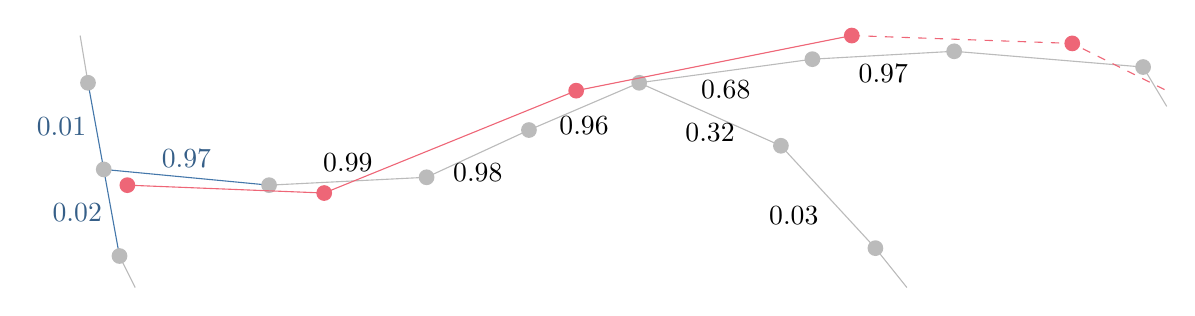
\begin{tikzpicture}
		% >>> street network
		\draw[blue] (-6.5,0.3) --node[blue!80!black,left] {$0.01$} (-6.3,-0.8);
		\draw[blue] (-6.1,-1.9) --node[blue!80!black,left] {$0.02$} (-6.3,-0.8);
		\draw[blue] (-4.2,-1) --node[blue!80!black,above] {$0.97$} (-6.3,-0.8);
		\draw[gray] (-4.2,-1) --node[black,above] {$0.99$} (-2.2,-0.9);
		\draw[gray] (-0.9,-0.3) --node[black,below] {$0.98$} (-2.2,-0.9);
		\draw[gray] (-0.9,-0.3) --node[black,below] {$0.96$} (0.5,0.3);
		\draw[gray] (2.7,0.6) --node[black,below] {$0.68$} (0.5,0.3);
		\draw[gray] (2.7,0.6) --node[black,below] {$0.97$} (4.5,0.7);
		\draw[gray] (2.3,-0.5) --node[black,below] {$0.32$} (0.5,0.3);
		\draw[gray] (2.3,-0.5) --node[black,below left] {$0.03$} (3.5,-1.8);
		\draw[gray] (-6.5,0.3) -- (-6.6,0.9);
		\draw[gray] (-6.1,-1.9) -- (-5.9,-2.3);
		\draw[gray] (3.5,-1.8) -- (3.9,-2.3);
		\draw[gray] (4.5,0.7) -- (6.9,0.5) -- (7.2,0);


		\fill[gray] (-6.5,0.3) circle (0.1);
		\fill[gray] (-6.3,-0.8) circle (0.1);
		\fill[gray] (-6.1,-1.9) circle (0.1);
		\fill[gray] (-4.2,-1) circle (0.1);
		\fill[gray] (-2.2,-0.9) circle (0.1);
		\fill[gray] (-0.9,-0.3) circle (0.1);
		\fill[gray] (0.5,0.3) circle (0.1);
		\fill[gray] (2.7,0.6) circle (0.1);
		\fill[gray] (4.5,0.7) circle (0.1);
		\fill[gray] (6.9,0.5) circle (0.1);
		\fill[gray] (2.3,-0.5) circle (0.1);
		\fill[gray] (3.5,-1.8) circle (0.1);
		% <<< street network

		% >>> track
		\fill[red] (-6,-1) circle (0.1);
		\fill[red] (-3.5,-1.1) circle (0.1);
		\fill[red] (-0.3,0.2) circle (0.1);
		\fill[red] (3.2,0.9) circle (0.1);
		\fill[red] (6,0.8) circle (0.1);
		\draw[red] (-6,-1) -- (-3.5,-1.1) -- (-0.3,0.2) -- (3.2,0.9);
		\draw[red,dashed] (3.2,0.9) -- (6,0.8) -- (7.2,0.2);
		% <<< track

	\end{tikzpicture}
	\caption{Sketch of the probabilities obtained during the search for the most probable path.
		The street network is drawn in gray (possible starting edges are drawn in blue) and calculated probabilities are printed above their edges.
		The recorded track is shown in red, the dashed line denotes the part of the track not yet considered by the algorithm.}
	\label{fig:sketch_overview}
\end{figure}

\section{Minimal distance from edge}
We need to calculate the minimal distance between a point at $(x,y)$ and an edge between points at $(x_0,y_0)$ and $(x_1,y_1)$, see \cref{fig:sketch_minimal_distance}.

\begin{figure}[ht]
	\centering
	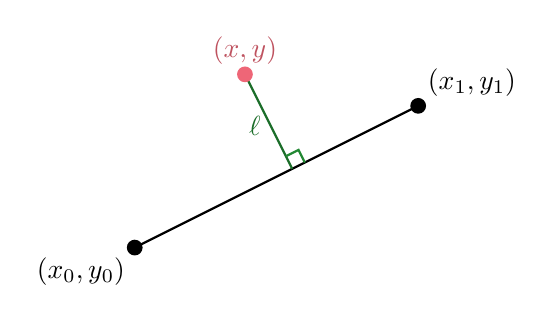
\begin{tikzpicture}
		\fill (1.6,0.8) circle (0.1);
		\node[anchor=south west] at (1.6,0.8) {$(x_1,y_1)$};
		\fill (-2,-1) circle (0.1);
		\node[anchor=north east] at (-2,-1) {$(x_0,y_0)$};
		\draw[thick] (1.6,0.8) -- (-2,-1);

		\draw[green!80!black, thick] (-0.6,1.2) -- node[pos=0.55,left] {$\ell$} (0,0);

		\fill[red] (-0.6,1.2) circle (0.1);
		\node[red!80!black, anchor=south] at (-0.6,1.2) {$(x,y)$};
		\draw[green, thick] (-0.08,0.16) -- ++(0.16,0.08) -- ++(0.08,-0.16);
	\end{tikzpicture}
	\caption{Sketch for the minimal distance between a point and an edge.}
	\label{fig:sketch_minimal_distance}
\end{figure}

The formula to calculate this is
%
\begin{align*}
	\ell(x,y,x_0,y_0,x_1,y_1)=\frac{|(y_1-y_0)x-(x_1-x_0)y+x_1y_0-x_0y_1|}{\sqrt{(y_1-y_0)^2+(x_1-x_0)^2}}\,,
\end{align*}
if the shortest distance is not to one of the nodes directly.
Considering this as well, we get
%
\begin{align*}
	 & \ell(x,y,x_0,y_0,x_1,y_1) \\
	 & \quad=
	\begin{cases}
		\sqrt{(y_0-y)^2+(x_0-x)^2}\,,                                                   & (x-x_0)(x_1-x_0)+(y-y_0)(y_1-y_0)<0\,, \\
		\sqrt{(y_1-y)^2+(x_1-x)^2}\,,                                                   & (x-x_1)(x_0-x_1)+(y-y_1)(y_0-y_1)<0\,, \\
		\frac{|(y_1-y_0)x-(x_1-x_0)y+x_1y_0-x_0y_1|}{\sqrt{(y_1-y_0)^2+(x_1-x_0)^2}}\,, & \text{else}\,.
	\end{cases}
\end{align*}

\section{Likelihood of a given edge}\label{sec:likelihood_of_edge}
As we want to obtain the most probable path in the street network, we need to define a probability of a certain edge being the correct one to identify a track point with.
We do this by considering the minimal distance between a point $p$ and an edge $e$, denoted $\ell(p,e)$.
The probability of an edge $e$ being the correct edge for point $p$ is then defined to decay exponentially with $\exp\big(\ell(p,e)\big)$, giving probabilities
%
\begin{align*}
	P(e|p) & = \left(\sum_{\text{edges }e'}\exp\Big(-\exp\big(\frac{\ell(p,e')}{5\unit{\metre}}\big)\Big)\right)^{-1}\exp\Big(-\exp\big(\frac{\ell(p,e)}{5\unit{\metre}}\big)\Big) \\
	       & = Z\exp\Big(-\exp\big(\frac{\ell(p,e)}{5\unit{\metre}}\big)\Big)\,,
\end{align*}
with partition function $Z$.\footnote{The denominator $5\unit{\metre}$ has been introduced to account for the rough accuracy of GPS, and to obtain a dimensionless quantity in the exponent.}
In practice, $Z$ is often hard to calculate, which is why we only work with the log-likelihood
%
\begin{align*}
	LL(p|e) = -\exp\big(\frac{\ell(p|e)}{5\unit{\metre}}\big)\,.
\end{align*}

Using log-likelihoods, we can obtain likelihood ratios, meaning that for point $p$, edge $e_1$ is $k$-times as likely as edge $e_2$ if
%
\begin{align*}
	\exp\big(LL(p|e_1)-LL(p|e_2)\big)=k\,.
\end{align*}

\section{Exploiting the graph structure}
Apart from the starting point, we always have a previous point, which has been associated with an edge.
Since we want our routes to follow the streets available in a street network (i.e. this does not work for cross-country running), we only need to consider the edges neighboring the edge of the previous point.
For these, we can calculate their weights as given in \cref{sec:likelihood_of_edge} and associate the current point with the edge with the highest likelihood.

We then update the likelihood of our current path, see \cref{sec:likelihood_path}, and repeat this step with the most likely path.

As mentioned, for the starting point in our track, we do not have a previous point, so this method does not work.
The workaround used for this is described in \cref{sec:starting_point}

\section{Starting point}\label{sec:starting_point}
For obtaining an edge associated to the starting point, we can not exploit the graph structure, as in principle, parts of the network far from each other can describe similarily good starting positions, see \cref{fig:starting_edge}.

\begin{figure}[ht]
	\centering
	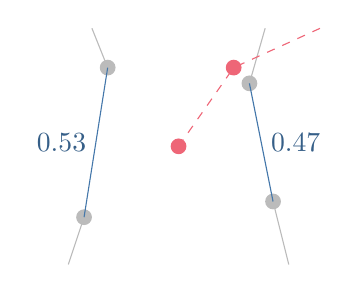
\begin{tikzpicture}
		% >>> street network
		\fill[gray] (-1,1) circle (0.1);
		\fill[gray] (-1.3,-0.9) circle (0.1);
		\draw[gray] (-1.2,1.5) -- (-1,1);
		\draw[gray] (-1.3,-0.9) -- (-1.5,-1.5);

		\fill[gray] (0.8,0.8) circle (0.1);
		\fill[gray] (1.1,-0.7) circle (0.1);
		\draw[gray] (1,1.5) -- (0.8,0.8);
		\draw[gray] (1.1,-0.7) -- (1.3,-1.5);
		% <<< street network

		% >>> possible starting edges
		\draw[blue] (-1.3,-0.9) -- node[blue!80!black,left] {$0.53$} (-1,1);
		\draw[blue] (0.8,0.8) -- node[blue!80!black,right] {$0.47$} (1.1,-0.7);
		% <<< possible starting edges

		% >>> track
		\fill[red] (-0.1,0) circle (0.1);
		\fill[red] (0.6,1) circle (0.1);
		\draw[red,dashed] (-0.1,0) -- (0.6,1) -- (1.7,1.5);
		% <<< track
	\end{tikzpicture}
	\caption{Sketch of the probabilities of different starting edges.
		The street network is drawn in gray (possible starting edges are drawn in blue) and calculated probabilites of possible starting edges are printed next to their edges.
		The recorded track is shown in red, the dashed line denotes the part of the track not yet considered by the algorithm.}
	\label{fig:starting_edge}
\end{figure}

We therefore have to consider all possible edges and obtain their probabilities as given in \cref{sec:likelihood_of_edge}.
We can then simply use these probabilities as we use the likelihoods for the remaining graph.

\section{Likelihood of a path}\label{sec:likelihood_path}
We already know how to extend the current most probable path by an edge.
If this new edge is a poor fit for the track point, the new most probable path might be an entirely different path.
We therefore need a measure to compare different paths to each other.
For this, we use the probabilities obtained for starting edges, and the weights obtained for all previous edges.

Formally, we can consider a path $\mathcal P=\left(e_1,\ldots,e_n\right)$ and a track $\mathcal T=\left(p_1,\ldots,p_m\right)$.
Here, a path consists of edges, and a track consists of points.
The log-likelihood of the track $\mathcal T$ under path $\mathcal P$ is then defined through
%
\begin{align*}
	LL(\mathcal P|\mathcal T)=\sum_{i=1}^nLL(e_i|p_i)
\end{align*}

Note that we define a likelihood even if $\mathcal P$ and $\mathcal T$ have different lengths.
This is necessary for intermediate steps in our algorithm, but we only halt the algorithm once we have obtained the most probable path with $|\mathcal P|=|\mathcal T|$.

\end{document}
